\section{Phân hệ Đặt hàng (Order)}

\subsection{Đặc tả Use Case}
Phân hệ Đặt hàng là hạt nhân nghiệp vụ của hệ thống BrewLite, chịu trách nhiệm chuyển hóa các sản phẩm trong giỏ hàng thành đơn hàng chính thức. Phân hệ tích hợp các dịch vụ tính giá (\texttt{PricingService}), kiểm tra và áp dụng khuyến mãi (\texttt{PromotionsService}), tích lũy điểm thành viên (\texttt{LoyaltyService}) và kiểm soát kho bằng khóa lạc quan (\texttt{Optimistic Locking}). Sơ đồ Use Case được minh họa tại Hình~\ref{fig:usecase-order}.

\begin{figure}[htbp]
    \centering
    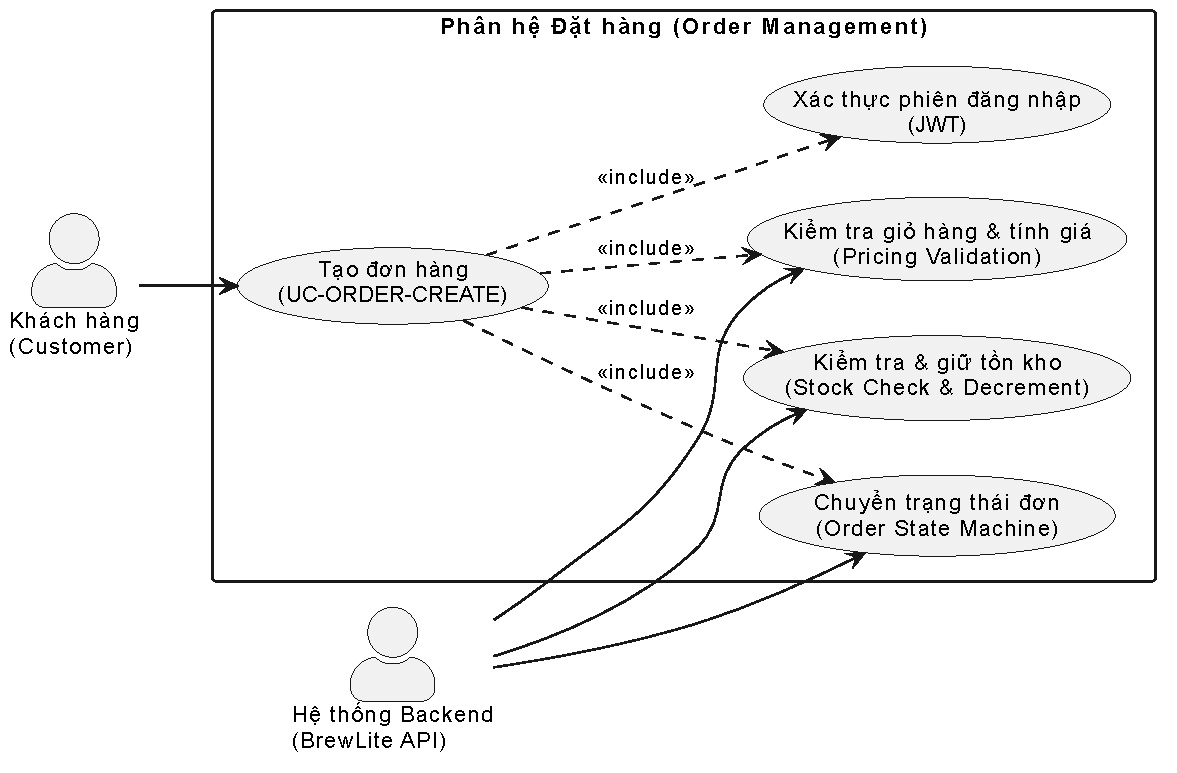
\includegraphics[width=0.75\textwidth]{figures/usecase-order.pdf}
    \caption{Sơ đồ Use Case - Phân hệ Đặt hàng}
    \label{fig:usecase-order}
\end{figure}

\begin{table}[htbp]
\centering
\small
\caption{Đặc tả Use Case: Tạo đơn hàng trực tuyến (UC-ORD-01)}
\label{tab:uc-spec-order}
\begin{tabularx}{\textwidth}{p{2.8cm}X}
\toprule
\textbf{Mục} & \textbf{Chi tiết Đặc tả} \\
\midrule
\textbf{Actor} & Khách hàng đã đăng nhập (Registered Customer) \\
\midrule
\textbf{Tiền điều kiện} & Khách hàng đã đăng nhập (mang Bearer JWT Token); giỏ hàng có ít nhất 1 sản phẩm. \\
\midrule
\textbf{Hậu điều kiện} & Bản ghi đơn hàng mới được tạo ở trạng thái \texttt{PENDING}; tồn kho sản phẩm được cập nhật; voucher được áp dụng; bản ghi lịch sử trạng thái được khởi tạo. \\
\midrule
\textbf{Luồng chính} & 
1. Khách hàng từ giỏ hàng nhấn "Tiến hành đặt hàng" đến trang Checkout (\texttt{/checkout}).\newline
2. Khách hàng nhập mã giảm giá (ví dụ \texttt{WELCOME10}) nếu có.\newline
3. Nhấn nút "Xác nhận đặt hàng".\newline
4. Giao diện gửi request \texttt{POST /api/v1/orders} kèm Bearer Token.\newline
5. Backend khởi động Interactive Transaction (\texttt{prisma.\$transaction}):\newline
\quad a. Kiểm tra từng sản phẩm, đối chiếu \texttt{version} và số lượng tồn kho \texttt{stock}.\newline
\quad b. Tính giá cơ bản, phụ thu size và giá topping qua \texttt{PricingService}.\newline
\quad c. Thẩm định mã giảm giá và tính số tiền giảm trừ qua \texttt{PromotionsService}.\newline
\quad d. Tính toán số điểm thưởng dự kiến tích lũy (\texttt{pointsEarned}).\newline
\quad e. Trừ tồn kho và tăng \texttt{version = version + 1} của sản phẩm.\newline
\quad f. Tạo bản ghi \texttt{orders}, các \texttt{order\_items} và \texttt{order\_item\_toppings}.\newline
\quad g. Thêm bản ghi vào \texttt{order\_status\_history} (chuyển trạng thái sang \texttt{PENDING}).\newline
6. Transaction commit thành công, trả về thông tin đơn hàng và mã số tự tăng \texttt{orderNumber} (ví dụ \#1042).\newline
7. Giao diện xóa giỏ hàng và điều hướng sang trang thanh toán (\texttt{/payment/[orderId]}). \\
\midrule
\textbf{Luồng ngoại lệ} & 
- Hết hàng hoặc tồn kho không đủ: Báo lỗi \texttt{400 Bad Request} ("Sản phẩm ... không đủ tồn kho"), rollback transaction.\newline
- Thiếu tồn kho hoặc xung đột phiên bản (Optimistic Lock Conflict): Báo lỗi \texttt{400 Bad Request} (\texttt{\"Insufficient stock or concurrent update...\"}), tự động rollback transaction.\newline
- Mã voucher không hợp lệ hoặc hết hạn: Báo lỗi \texttt{400 Bad Request} ("Mã giảm giá không hợp lệ").\newline
- Chưa đăng nhập: Báo lỗi \texttt{401 Unauthorized}, điều hướng về trang đăng nhập. \\
\bottomrule
\end{tabularx}
\end{table}

\subsection{Sơ đồ Hoạt động (Activity Diagram)}
Luồng hoạt động kiểm tra điều kiện tồn kho, tính giá và cam kết giao dịch tạo đơn được biểu diễn tại Hình~\ref{fig:activity-order}.

\begin{figure}[htbp]
    \centering
    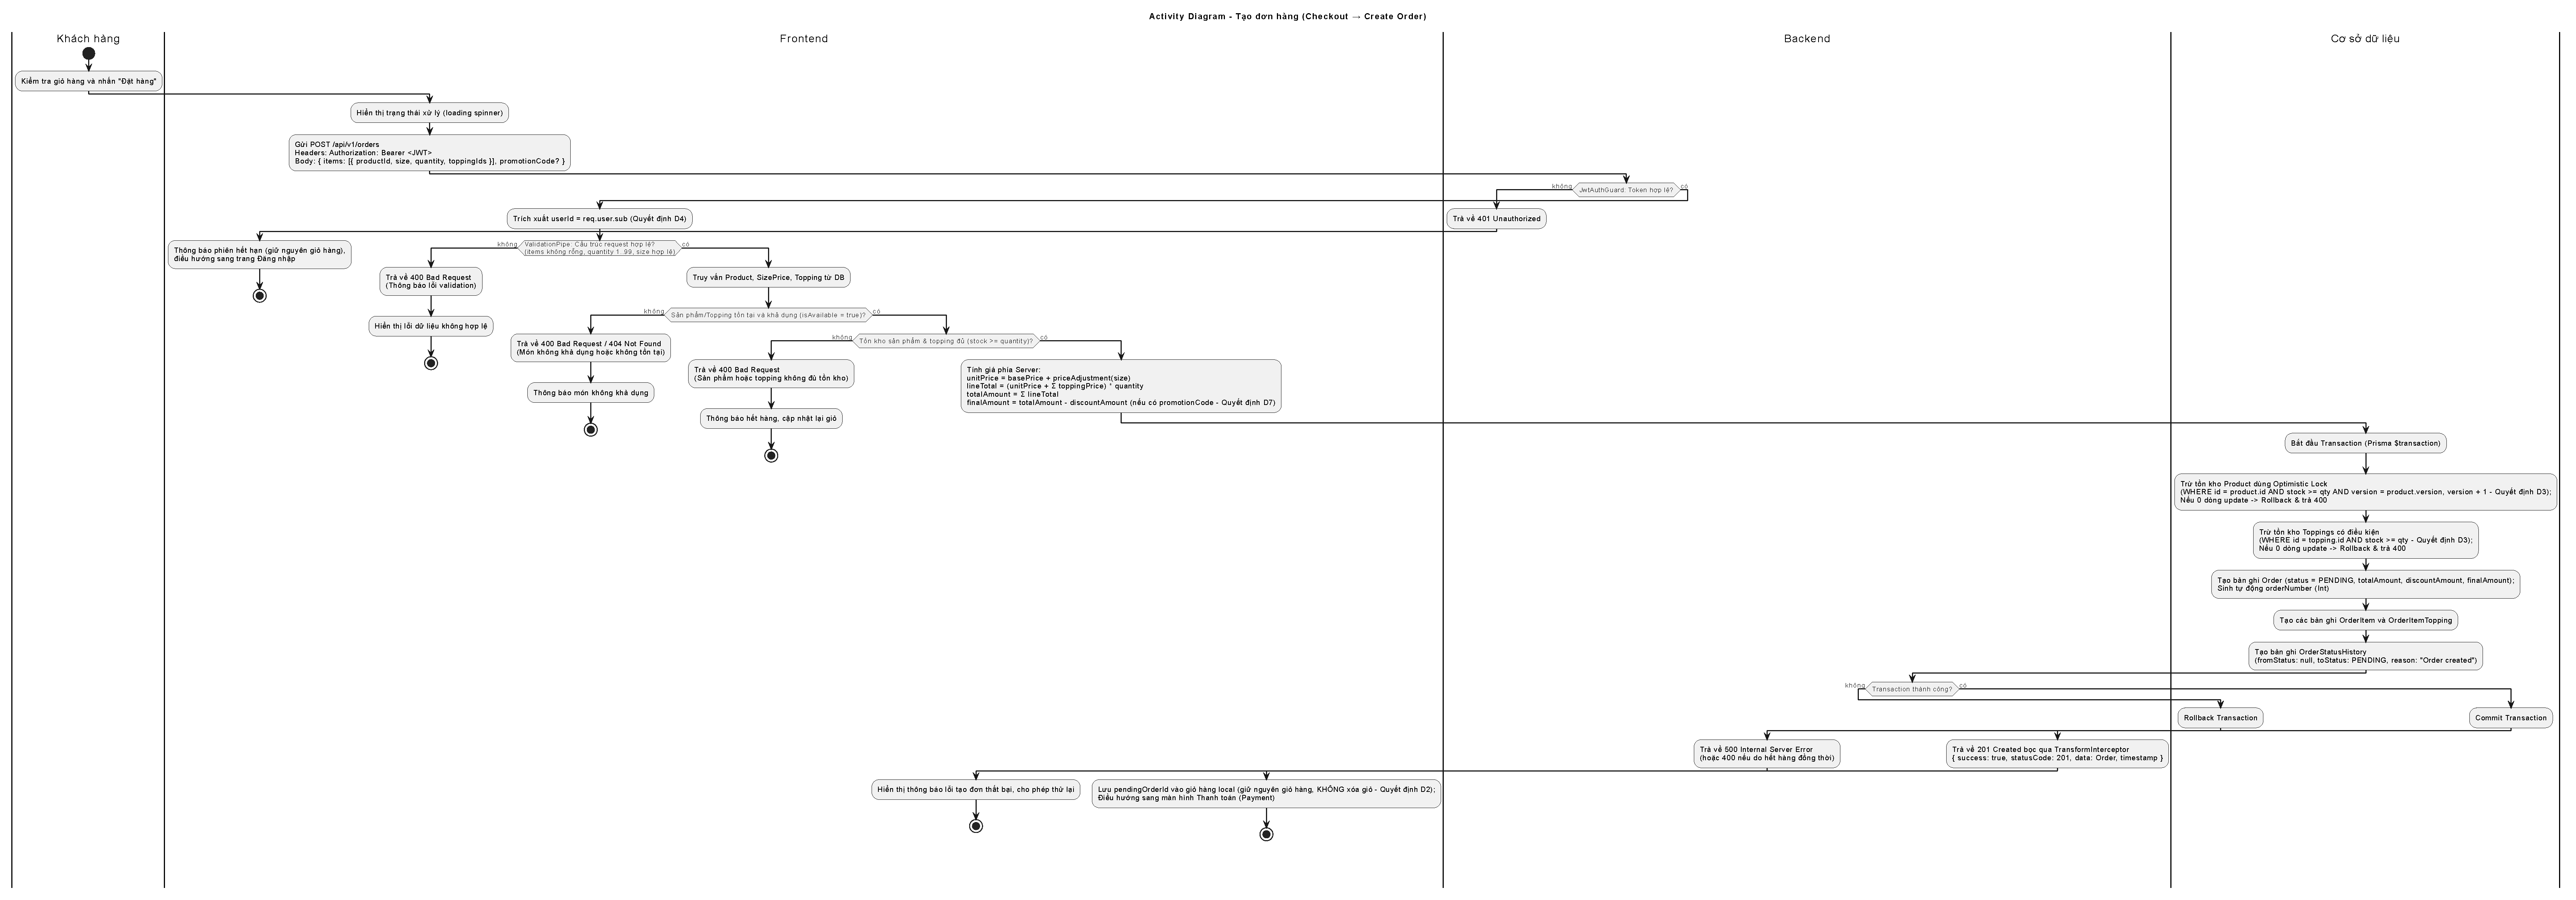
\includegraphics[width=0.75\textwidth]{figures/activity-order.pdf}
    \caption{Sơ đồ Hoạt động - Phân hệ Đặt hàng}
    \label{fig:activity-order}
\end{figure}

\subsection{Sơ đồ Tuần tự (Sequence Diagram)}
Sơ đồ Tuần tự minh họa chi tiết toàn bộ các lời gọi dịch vụ phối hợp trong một transaction tạo đơn hàng tại Hình~\ref{fig:sequence-order}.

\begin{figure}[htbp]
    \centering
    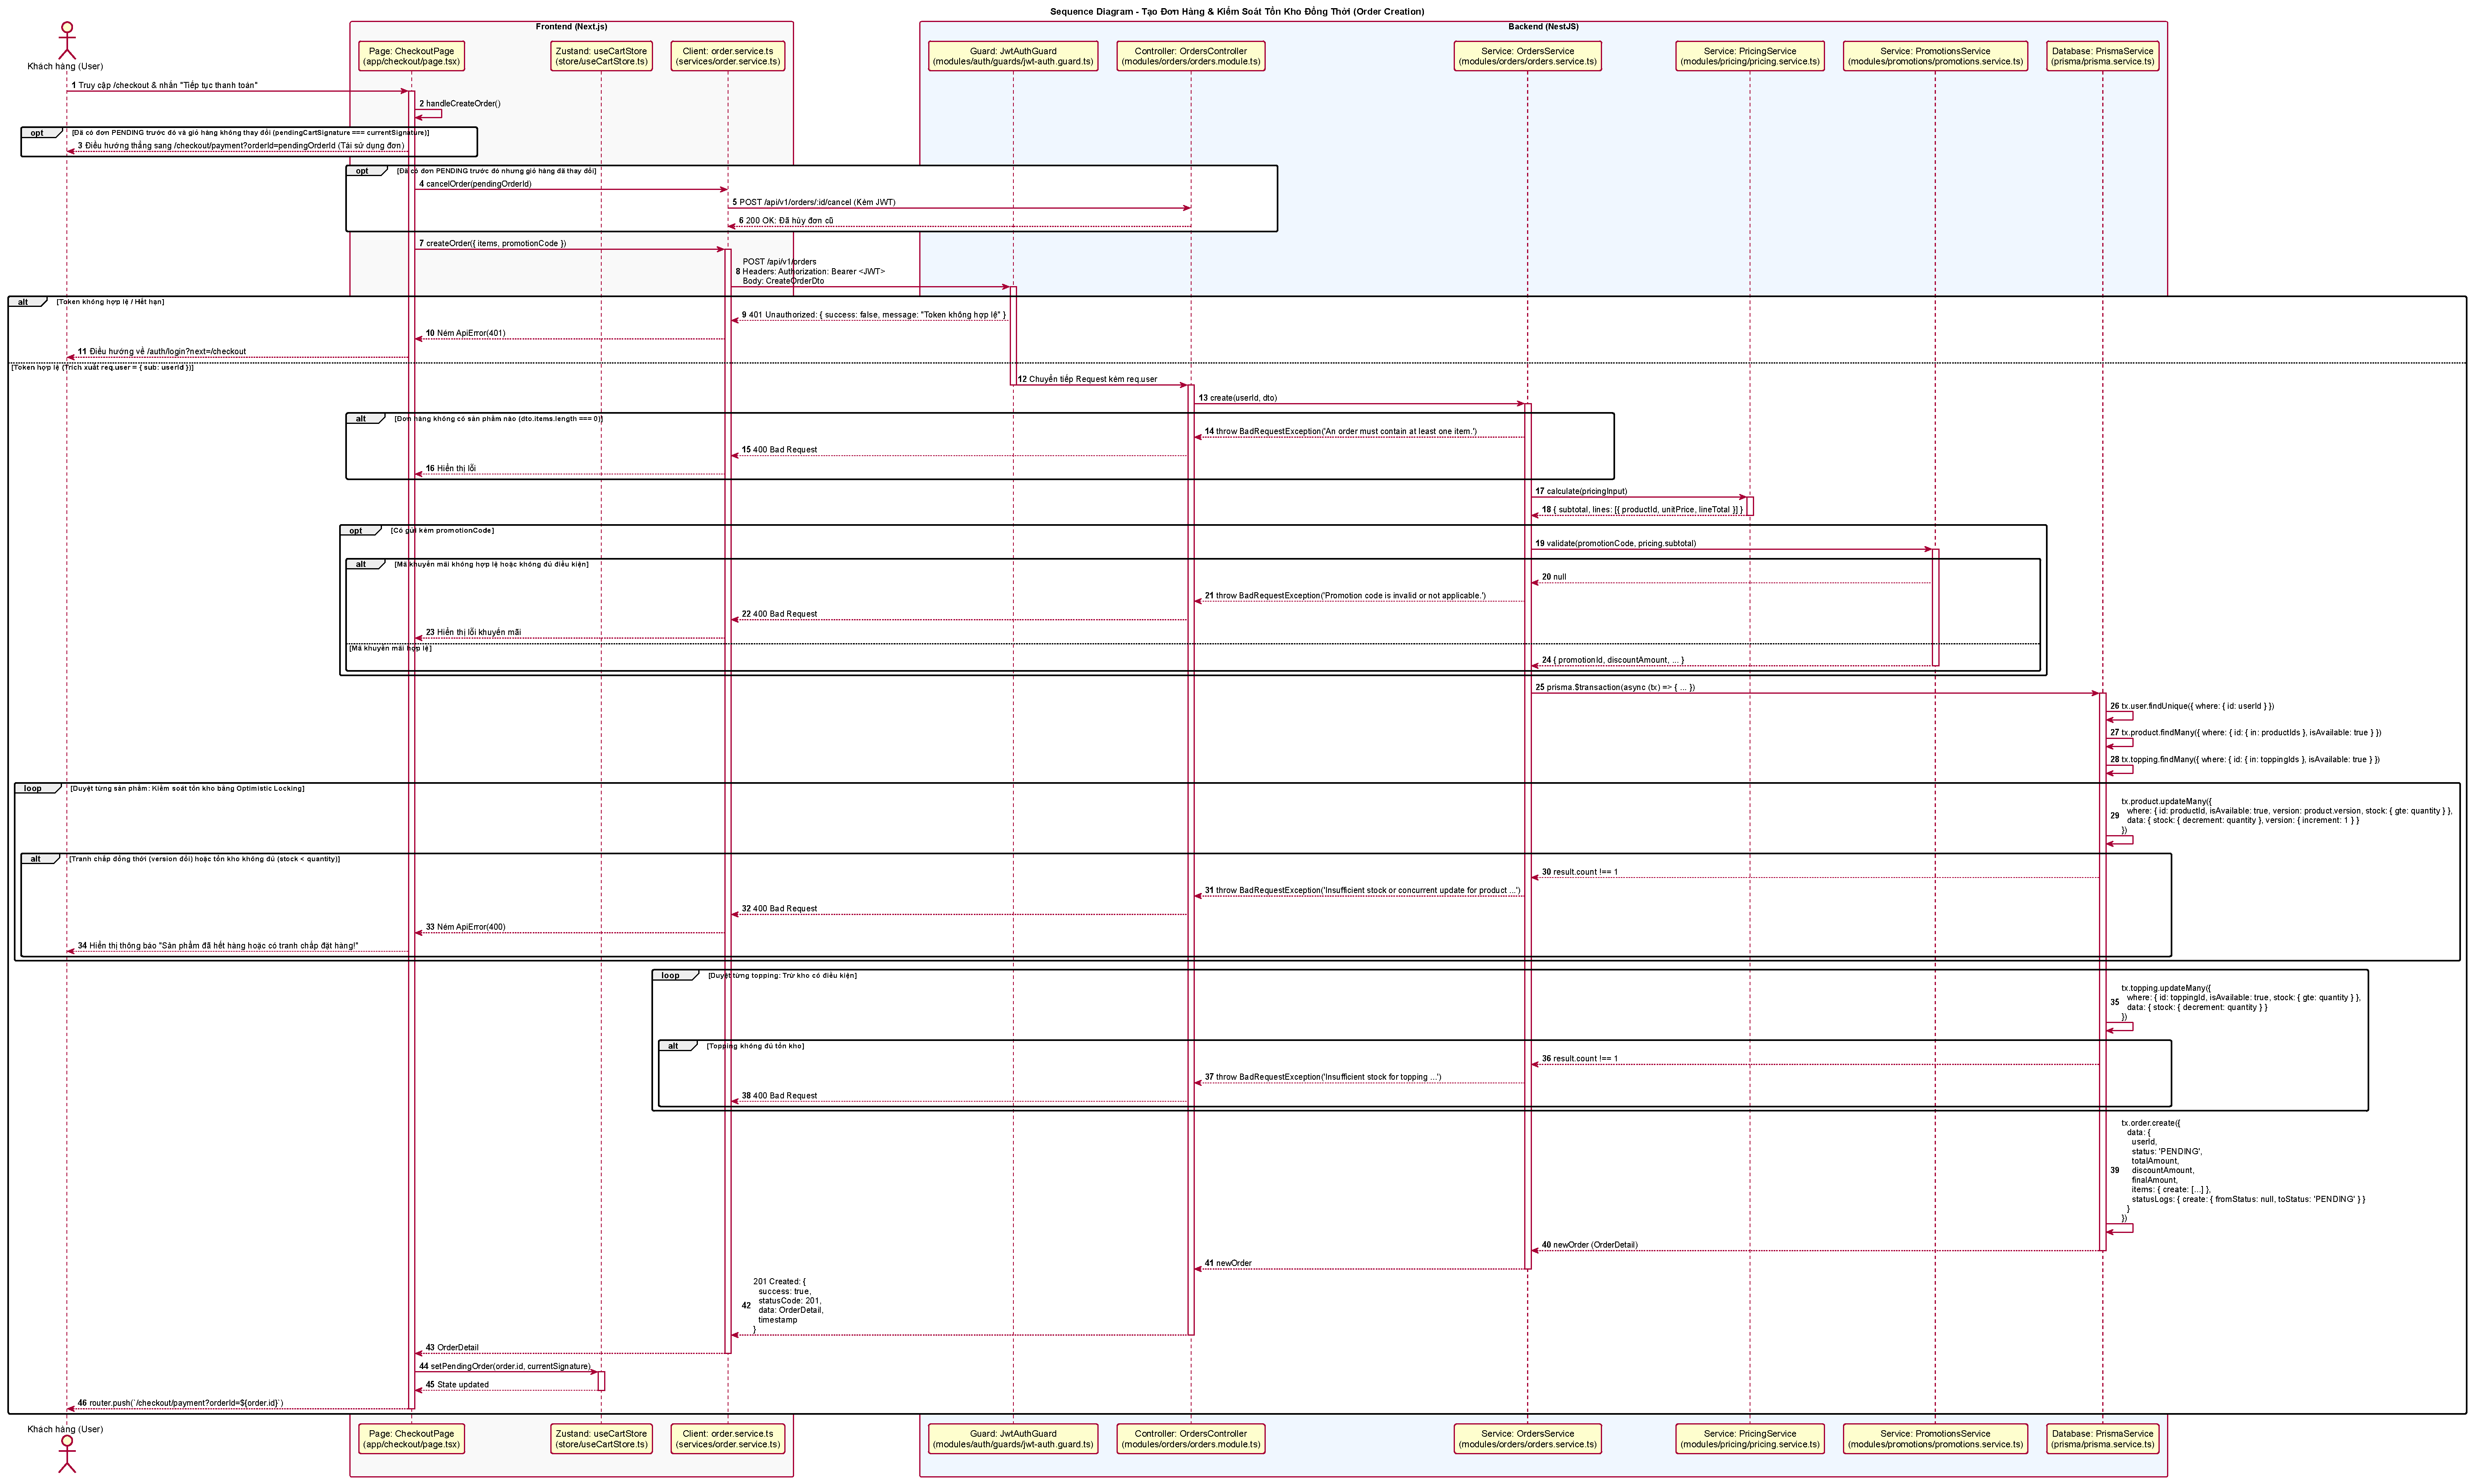
\includegraphics[width=0.9\textwidth]{figures/sequence-order.pdf}
    \caption{Sơ đồ Tuần tự - Phân hệ Đặt hàng (Interactive Transaction \& Pricing Engine)}
    \label{fig:sequence-order}
\end{figure}

\subsection{Hợp đồng API (API Contract)}
\begin{table}[htbp]
\centering
\small
\caption{Danh mục API Endpoints - Phân hệ Đặt hàng}
\label{tab:api-order}
\begin{tabularx}{\textwidth}{llp{4.5cm}X}
\toprule
\textbf{Phương thức} & \textbf{Endpoint} & \textbf{Mô tả Request Payload} & \textbf{Phản hồi chính} \\
\midrule
\texttt{POST} & \texttt{/api/v1/orders} & 
\texttt{\{items: [\{productId, size, quantity, toppings\}], promotionCode?\}} (Header: \texttt{Authorization: Bearer <JWT>}) & 
\texttt{201 Created}: Trả về đơn hàng mới tạo với cấu trúc bọc chuẩn \texttt{TransformInterceptor}. Lỗi: \texttt{400 Bad Request}, \texttt{401 Unauthorized}. \\
\texttt{GET} & \texttt{/api/v1/orders/:id} & Tham số \texttt{id} của đơn hàng (Header: Bearer Token) & 
\texttt{200 OK}: Chi tiết đơn hàng, danh sách món, trạng thái xử lý và các lần thử thanh toán. \\
\bottomrule
\end{tabularx}
\end{table}

\subsection{Ánh xạ Cơ sở dữ liệu (Database Mapping)}
Quá trình tạo đơn hàng thực thi nguyên tử trong một \texttt{prisma.\$transaction}:
\begin{lstlisting}[language=SQL]
-- 1. Kiem tra va cap nhat ton kho voi Optimistic Locking
UPDATE products 
SET stock = stock - :quantity, version = version + 1
WHERE id = :productId AND version = :currentVersion AND stock >= :quantity;

-- 2. Tao ban ghi don hang chinh thuc
INSERT INTO orders (id, order_number, user_id, status, total_amount, discount_amount, final_amount, points_earned, version, created_at, updated_at)
VALUES (cuid(), nextval('orders_order_number_seq'), :userId, 'PENDING', :totalAmount, :discountAmount, :finalAmount, :pointsEarned, 0, NOW(), NOW());

-- 3. Tao cac chi tiet don hang va luu snapshot gia
INSERT INTO order_items (id, order_id, product_id, size, quantity, unit_price, line_total)
VALUES (cuid(), :orderId, :productId, :size, :quantity, :unitPrice, :lineTotal);

-- 4. Ghi nhat ky trang thai ban dau
INSERT INTO order_status_history (id, order_id, from_status, to_status, changed_by, created_at)
VALUES (cuid(), :orderId, NULL, 'PENDING', 'system', NOW());
\end{lstlisting}

\subsection{Kịch bản Kiểm thử (Test Cases)}
\begin{table}[htbp]
\centering
\small
\caption{Tóm lược các Ca kiểm thử tiêu biểu - Phân hệ Đặt hàng}
\label{tab:tc-order}
\begin{tabularx}{\textwidth}{llp{2.6cm}p{3cm}Xc}
\toprule
\textbf{Mã TC} & \textbf{Loại} & \textbf{Tiền điều kiện} & \textbf{Endpoint / Màn hình} & \textbf{Kết quả mong đợi} & \textbf{Trạng thái} \\
\midrule
\texttt{TC-ORD-API-01} & Hợp lệ & Đủ tồn kho, có token & \texttt{POST /orders} & HTTP 201, tạo đơn trạng thái PENDING, trừ kho & Chưa chạy \\
\texttt{TC-ORD-API-03} & Lỗi & Tồn kho không đủ & \texttt{POST /orders} & HTTP 400, rollback transaction, không trừ kho & Chưa chạy \\
\texttt{TC-ORD-API-04} & Lỗi & Xung đột version (Optimistic) & \texttt{POST /orders} & HTTP 400 Bad Request (\"Insufficient stock or concurrent update...\"), rollback & Đạt \\
\texttt{TC-ORD-API-06} & Hợp lệ & Áp voucher WELCOME10 & \texttt{POST /orders} & Giảm 10\% (tối đa 20k), finalAmount chính xác & Đạt \\
\texttt{TC-ORD-UI-01} & Giao diện & Đã đăng nhập & Trang \texttt{/checkout} & Hiển thị tóm tắt đơn, ô nhập voucher và nút đặt & Chưa chạy \\
\bottomrule
\end{tabularx}
\end{table}

\subsection{Giao diện Người dùng}
\begin{figure}[htbp]
    \centering
    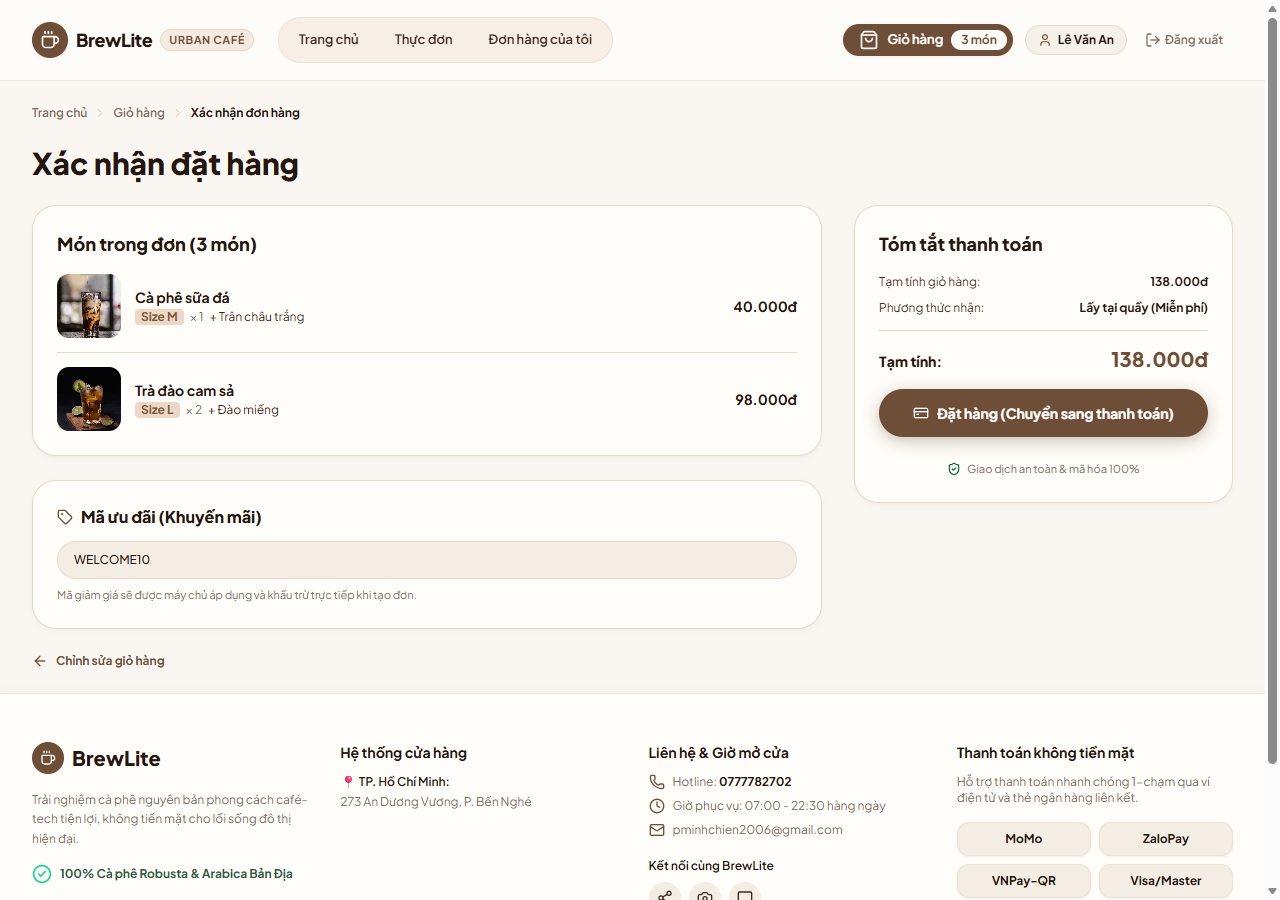
\includegraphics[width=0.92\textwidth]{figures/ui-checkout.png}
    \caption{Giao diện Xác nhận Đặt hàng và Áp dụng Khuyến mại}
    \label{fig:ui-order}
\end{figure}
